%%%%%%%%%%%%%%%%%%%%%%%%%%%%%%%%%%%%%%%%%%%%%%%%%%%%%%%%%%%%%%%%%%%%%%%%%%%%%%%
%% Active Learning Machine Learning Methodology
%%
%%
%% Points to mention:
%%    Voronoi is used because it is insensitive to volume expansions of structure
%%    Explain PCA analysis
%%    TEMP
%%
%% TODO:
%%    Why AB2 and AB3
%%    TEMP
%%%%%%%%%%%%%%%%%%%%%%%%%%%%%%%%%%%%%%%%%%%%%%%%%%%%%%%%%%%%%%%%%%%%%%%%%%%%%%%

% ################################# Paragraph #################################
% %%%%%%%%%%%%%%%%%%%%%%%%%%%%%%%%%%%%%%%%%%%%%%%%%%%%%%%%%%%%%%%%%%%%%%%%%%%%%
% TEMP
% %%%%%%%%%%%%%%%%%%%%%%%%%%%%%%%%%%%%%%%%%%%%%%%%%%%%%%%%%%%%%%%%%%%%%%%%%%%%%
% Data prep. | Unique Structures | Atom subst., V relax | Fingerprinting
The structures that comprise the candidate data set were constructed by parsing for structurally unique systems in the OQMD and Materials Project DFT databases.
The structural uniqueness was performed using a space-group symmetry classification scheme developed by TEMP-Ankit-REF which can classify any arbitrary structure based on stoichiometry (composition), space-group, and Wyckoff positioning of the atoms
 (see SI for more details on the structural classification scheme).
To focus the scope of the study, only AB2 and AB3 stoichiometries were parsed from the databases.
The AB2 formula was chosen because it includes \rIrOtwo, the known most stable polymorph of IrO2.
Importantly, AB3 was chosen to include high valency IrO3 structures in our search.
This classification scheme can directly serve as a fingerprinting scheme and has successfully been used for the prediction of formation energies.  % REF Ankit paper
The results of the classification scheme resulted in a XYZ AB2 and XYZ AB3 structural prototypes for which iridium and oxygen were replaced for A and B sites, respectively.
Finally, a coarse isotropic volume relaxation based on atomic radii was performed on the structures to accommodate the atomic radii of iridium and oxygen into the lattice.
Finally, a Voronoi tessellation based fingerprinting scheme developed by Wolverton-paper-REF was used to encode the relevant chemical information for each structure.
The Voronoi based method was used because it is insensitive to volume relaxation.
PCA was used to reduce the dimensionality of the feature space from 271  to 20 features such that 99percent of the variance is captured.


% ################################# Paragraph #################################
% %%%%%%%%%%%%%%%%%%%%%%%%%%%%%%%%%%%%%%%%%%%%%%%%%%%%%%%%%%%%%%%%%%%%%%%%%%%%%
% TEMP
% %%%%%%%%%%%%%%%%%%%%%%%%%%%%%%%%%%%%%%%%%%%%%%%%%%%%%%%%%%%%%%%%%%%%%%%%%%%%%
% Iterative Training of Gaussian Process
The active learning algorithm proceeds through iterative ML training, prediction, and acquisition steps and is visualized in figure TEMP.
The
A Gaussian process (GP) regression employing a rational quadratic kernel was chosen as the ML model because it offers a high degree of flexibility and importantly, error quantification for the predicted formation energies.
Further details on the GP model, including hyper parameter information, is including in the SI.


\begin{enumerate}
  \item Candidate space of structures is generated
  \item Initial seed data is used to train a ML model
  \item ML model predicts energy of entire candidate space
  \item Most valuable calculation(s) is selected using acquisition function
  \item DFT calculation(s) is(are) performed to obtain additional training data points
  \item ML model is retrained with additional data
  \item Repeat steps (TEMP) through (TEMP) until convergence criteria is reached
  % \item TEMP
\end{enumerate}

% - Trained Gaussian Process, rational quadratic kernel, variable length scales.
% CV error of XYZ eV/atom, initial predictions in figure XYZ.
% - Selected 10 structures with lowest prediction-uncertainty for DFT.
% Structures were volume optimized, then fully relaxed, described in methods XYZ.
% - Model retrained with the 10 DFT computed structures ONLY, 271 features->110 features applicable to \ce{IrO_2}->20 principle components for 99.9 percent variance.
% CV error…
% - Repeat until XYZ, final predictions shown in Fig XYZ



% | - Figure | Active Learning Algorithm
\begin{figure*}
\centering
\makebox[\textwidth][c]{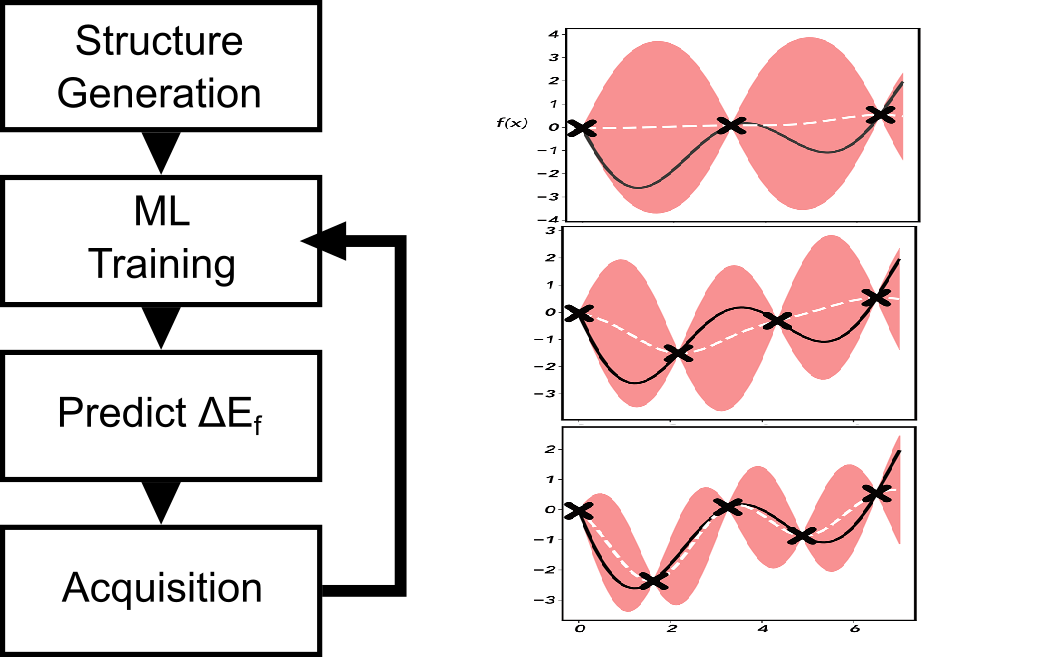
\includegraphics
  {02_figures/Surrogate_model_mine.png}
  }
\caption{\label{fig:all_diagram}
(a) Active learning algorithm diagram.
First the candidate space of structures is generated,
next, the machine learning model is trained on any available DFT formation energy data.
The trained ML model is then used to predict the DE of the entire candidate space.
Finally, an acquisition step is performed to pick the next most valuable calculation to perform an-initio DFT on
% -----------------------------------------------------------------------------
(b) Toy model demonstrating a GP model converging with each subsequent iteration.
% -----------------------------------------------------------------------------
}
\end{figure*}
% __|



% | - __old__
% ################################# Paragraph #################################
% AB2 Structures Ankit
% - There are XYZ unique AB2 structures (or multiples, e.g. A2B4)
% - Of those we found 697 unique AB2 prototypes (unique SG/Wyckoff combination) in OQMD/MP
% - To generate our test set we substituted Ir for A and O for B, then isotropically expanded cell volume to constrain a minimum Ir-O distance of XYZ
% - Next translated each of the 697 structures to be described by 271 features (invariant to isotropic expansion/compression), then reduced to 30 using PCA, described in methods XYZ
% - To generate initial training data use existing DFT. Not enough on \ce{IrO_2}, so used OQMD to generate initial training data from nearest structures in phase space, described in Methods XYZ. Training set of 30 structures in SI XYZ.
% __|
